% !TEX TS-program = XeLaTeX
% use the following command: 
% $ xelatex -shell-escape -output-driver="xdvipdfmx -z 0" article.tex
% this "-z 0" must be used to suppress compression in XMP Metadata packet 
% all document files must be coded in UTF-8
\documentclass{textolivre}
% for anonymous submission
%\documentclass[anonymous]{textolivre}
% to create HTML use 
%\documentclass{textolivre-html}
% remove all auxiliary files
% find . -name 'article.*' ! -name '*.tex' ! -name '*.pdf' ! -name '*.bib' ! -name '*.html' -type f -exec rm {} \;
% HTML compile using make4ht
% $ make4ht -c textolivre-html.cfg -u -x article "fn-in,svg,pic-align"   
% $ make4ht -c textolivre-html.cfg -u -x article "fn-in,mathml,mathjax"   # use `mathjax' instead of `svg' to get LaTeX equation that will be handled by MathJax
% $ bibtex article
% clean and prettify HTML 
% $ tidy -o article-tidy.html --output-xhtml --break-before-br --wrap 0 article.html 2> errs.txt
% https://www.html-tidy.org/documentation/

% Metadata
\begin{filecontents*}{article.xmpdata}
    \Title{Crisos socioecológica y comunicación durante la Marea Roja de Chiloé (2016)}
    \Author{Jorge Valdebenito Allendes}
    \Language{es}
    \Keywords{Crisis \sep Comunicación \sep Socioecología \sep Interdisciplina \sep Sistemas \sep Marxismo}
    \Journaltitle{Texto Livre}
    \Journalnumber{1983-3652}
    \Volume{14}
    \Issue{1}
    \Firstpage{1}
    \Lastpage{18}
    \Doi{10.35699/1983-3652.2021.26231}

    \setRGBcolorprofile{sRGB_IEC61966-2-1_black_scaled.icc}
            {sRGB_IEC61966-2-1_black_scaled}
            {sRGB IEC61966 v2.1 with black scaling}
            {http://www.color.org}
\end{filecontents*}

% PDF/A
% - install package icc-profiles
% - it is necessary to convert all image files to PDF/A
%   use ghostscript as shown below:
%   PDF images:
%   $ gs -dPDFA -dBATCH -dNOPAUSE -sColorConversionStrategy=UseDeviceIndependentColor -dCompatibilityLevel=1.4 -sDEVICE=pdfwrite -sProcessColorModel=DeviceCMYK -dPDFACompatibilityPolicy=2 -sOutputFile=figure-a.pdf figure.pdf
%   Other images:
%   $ convert figure.png figure.eps
%   $ gs -dPDFA -dBATCH -dNOPAUSE -sColorConversionStrategy=UseDeviceIndependentColor -dCompatibilityLevel=1.4 -sDEVICE=pdfwrite -sProcessColorModel=DeviceCMYK -dPDFACompatibilityPolicy=2 -dEPSCrop -sOutputFile=figure.pdf figure.eps
%   # script to convert all files:
%   $ for img in $( ls figure*.png ); do convert $img ${img%png}eps; gs -dPDFA -dBATCH -dNOPAUSE -sColorConversionStrategy=UseDeviceIndependentColor -dCompatibilityLevel=1.4 -sDEVICE=pdfwrite -sProcessColorModel=DeviceCMYK -dPDFACompatibilityPolicy=2 -dEPSCrop -sOutputFile=${img%png}pdf ${img%png}eps; done

\journalname{Texto Livre: Linguagem e Tecnologia}
\thevolume{14}
\thenumber{1}
\theyear{2021}
\receiveddate{\DTMdisplaydate{2020}{05}{21}{-1}} % YYYY MM DD
\accepteddate{\DTMdisplaydate{2020}{08}{31}{-1}}
\publisheddate{\DTMdisplaydate{2020}{11}{16}{-1}}
% Corresponding author
\corrauthor{Jorge V. Allendes}
% DOI
\articledoi{10.35699/1983-3652.2021.26231}
% Abbreviated author list for the running footer
\runningauthor{Allendes}

\title{Crisos socioecológica y comunicación durante la Marea Roja de Chiloé (2016)}
\othertitle{Crise sócio-ecológica e comunicação durante a Maré Vermelha de Chiloé (2016)}
\othertitle{Socioecological crisis and communications during the Red Tide of Chiloé (2016)}

\author[1]{Jorge Valdebenito Allendes \orcid{0000-0003-3249-1855} \thanks{Email: \url{jorge.valdebenito@postgrado.uv.cl}}}
\affil[1]{Universidad de Valparaíso, Chile.}

%\usepackage[backend=biber,style=abnt, ittitles]{biblatex}
%\DeclareLanguageMapping{brazil}{brazil-apa}
\addbibresource{article.bib}     
% use biber instead of bibtex
% $ biber tl-article-template
% $ pdflatex tl-article-template.tex

% set language of the article
\setdefaultlanguage{spanish}
\setotherlanguage[variant=brazilian]{portuguese}
\setotherlanguage{english}

\usepackage{multirow}

\begin{document}
\maketitle

\begin{polyabstract}
\begin{abstract}
¿Qué rol asumen los medios de comunicación durante el transcurso de las
coyunturas de conflicto social en Chile? Delimitando a la crisis socioecológica de Chiloé
del año 2016, se presenta un análisis del contenido de las proyecciones televisivas sobre
sus principales hitos. Esto se realiza siguiendo un diseño muestral formulado para la
comparación empírica del material periodístico, acorde a sus criterios normativos,
plataforma de circulación y fase coyuntural. Teóricamente el análisis integra rendimientos
provenientes de perspectivas luhmannianas y marxistas sobre la crisis, comunicación y
relaciones socioecológicas. De conjunto, se articula un producto interdisciplinario de
ciencias sociales y de la comunicación. Sus resultados problematizan la sucesión de
colisiones de expectativas cognitivo-normativas, o en otros términos, el transcurso de las
batallas ideológicas durante un episodio abierto de lucha de clases.

\keywords{Crisis \sep Comunicación \sep Socioecología \sep Interdisciplina \sep Sistemas \sep Marxismo.}
\end{abstract}

\begin{portuguese}
\begin{abstract}
Qual o papel que a mídia assume ao longo dos tempos de conflito social no
Chile? Delimitando a crise socioecológica de Chiloé em 2016, é apresentada uma análise
do conteúdo das projeções televisivas sobre seus principais marcos. Isso é feito a partir
de um desenho amostral formulado para a comparação empírica do material jornalístico,
de acordo com seus critérios normativos, plataforma de circulação e fase conjuntural.
Teoricamente, a análise integra retornos das perspectivas luhmanniana e marxista sobre
crise, comunicação e relações socioecológicas. Ao todo, articula-se um produto
interdisciplinar das ciências sociais e da comunicação. Seus resultados problematizam a
sucessão de choques de expectativas cognitivo-normativas, ou, em outras palavras, o
curso das batalhas ideológicas durante um episódio aberto de luta de classes.

\keywords{Crise \sep Comunicação \sep Socioecologia \sep Interdisciplina \sep Sistemas \sep Marxismo.}
\end{abstract}
\end{portuguese}

\begin{english}
\begin{abstract}
What role does the media assume during social conflicts in Chile? Delimiting
to the socio-ecological crisis of Chiloé in 2016, this study set out to present a content
analysis of the television broadcast covering its main milestones. Data for this study were
collected using a sampling design formulated for the empirical comparison of journalistic
material based on its normative criteria, type of media, and stage of development.
Theoretically, the analysis integrates Luhmannian and Marxist p erspectives on the crisis,
communication, and socio-ecological relations. As a whole, it articulates an
interdisciplinary product of social sciences and communication. Its results problematize the
succession of collisions of cognitive-normative expectations, or in other words, the
unfolding of ideological battles during an episode of class struggle.

\keywords{Crisis \sep Communication \sep Socio-ecology \sep Interdiscipline \sep Systems \sep Marxism.}
\end{abstract}
\end{english}

\end{polyabstract}


\section{Introducción}\label{sec-intro}
Diversos estudios sostienen que el mundo contemporáneo se encuentra
atravesado por la incompatibilidad temporal entre la reproducción metabólica del
ecosistema, y la configuración política de su ciclo económico \cite{arboleda,Mascareo2018}.
Según los antecedentes, las medidas tendientes a diseñar
estrategias de conciliación o equilibrio entre dichos procesos han sido insuficientes
\cite{Folke2016}. Expresión de ello es el sostenido deterioro de la biomasa planetaria,
asociada comúnmente a la expansión e intensificación de la producción industrial \cite{ipcc2013,Kamjunke2017}. 
Según algunos tal situación ha originado una nueva fase
geológica, denominada como ‘antropoceno’ \cite{Foster2016}. Rol clave juega la
proyección mediática en la divulgación del conocimiento sobre sus causas,
comportamiento, y futuras proyecciones \cite{billi2017}. Las críticas al
respecto sostienen que dicho proceso se encuentra ideológicamente instrumentalizado
por quienes poseen la propiedad de los medios de comunicación contemporáneos
\cite{Gunderson2019}.

La relevancia de la comunicación de masas en la sociedad moderna se encuentra
dada por su aspecto diferencial respecto de las formaciones sociales pretéritas
\cite{Habermas2006}. De ahí que el presente estudio proponga como objetivo central
examinar el rol que asumen medios como la televisión abierta durante la apertura de
coyunturas de conflicto socioecológico. Como caso de estudio se considera pertinente el
‘mayo chilote’, ocurrido durante el año 2016 en la isla de Chiloé \cite{ValdebenitoAllendes2018}.
Ubicada al sur de Chile -- entre los paralelos 42 y 43 y los meridianos 74 y 73 (\Cref{fig01})
--, tal episodio comprendió la articulación de un colapso ambiental y levantamiento
popular \cite{cabello2018,roman2016}. Las fuentes de los
sucesos permanecen hasta hoy sin determinación científica \cite{buschmann2016,t13b}. 
El caso estuvo marcado por tres acontecimientos: i) inusual extensión
temporal y geográfica de los efectos asociados a una marea roja \cite{burrows2016}; ii)
gigantesca varazón de fauna marina en las costas de Cucao --sureste de la isla-- \cite{cnnchile2016b}; 
y iii) violentas manifestaciones populares, protagonizadas por sectores de
la pesca artesanal.

\begin{figure}[htbp]
 \centering
 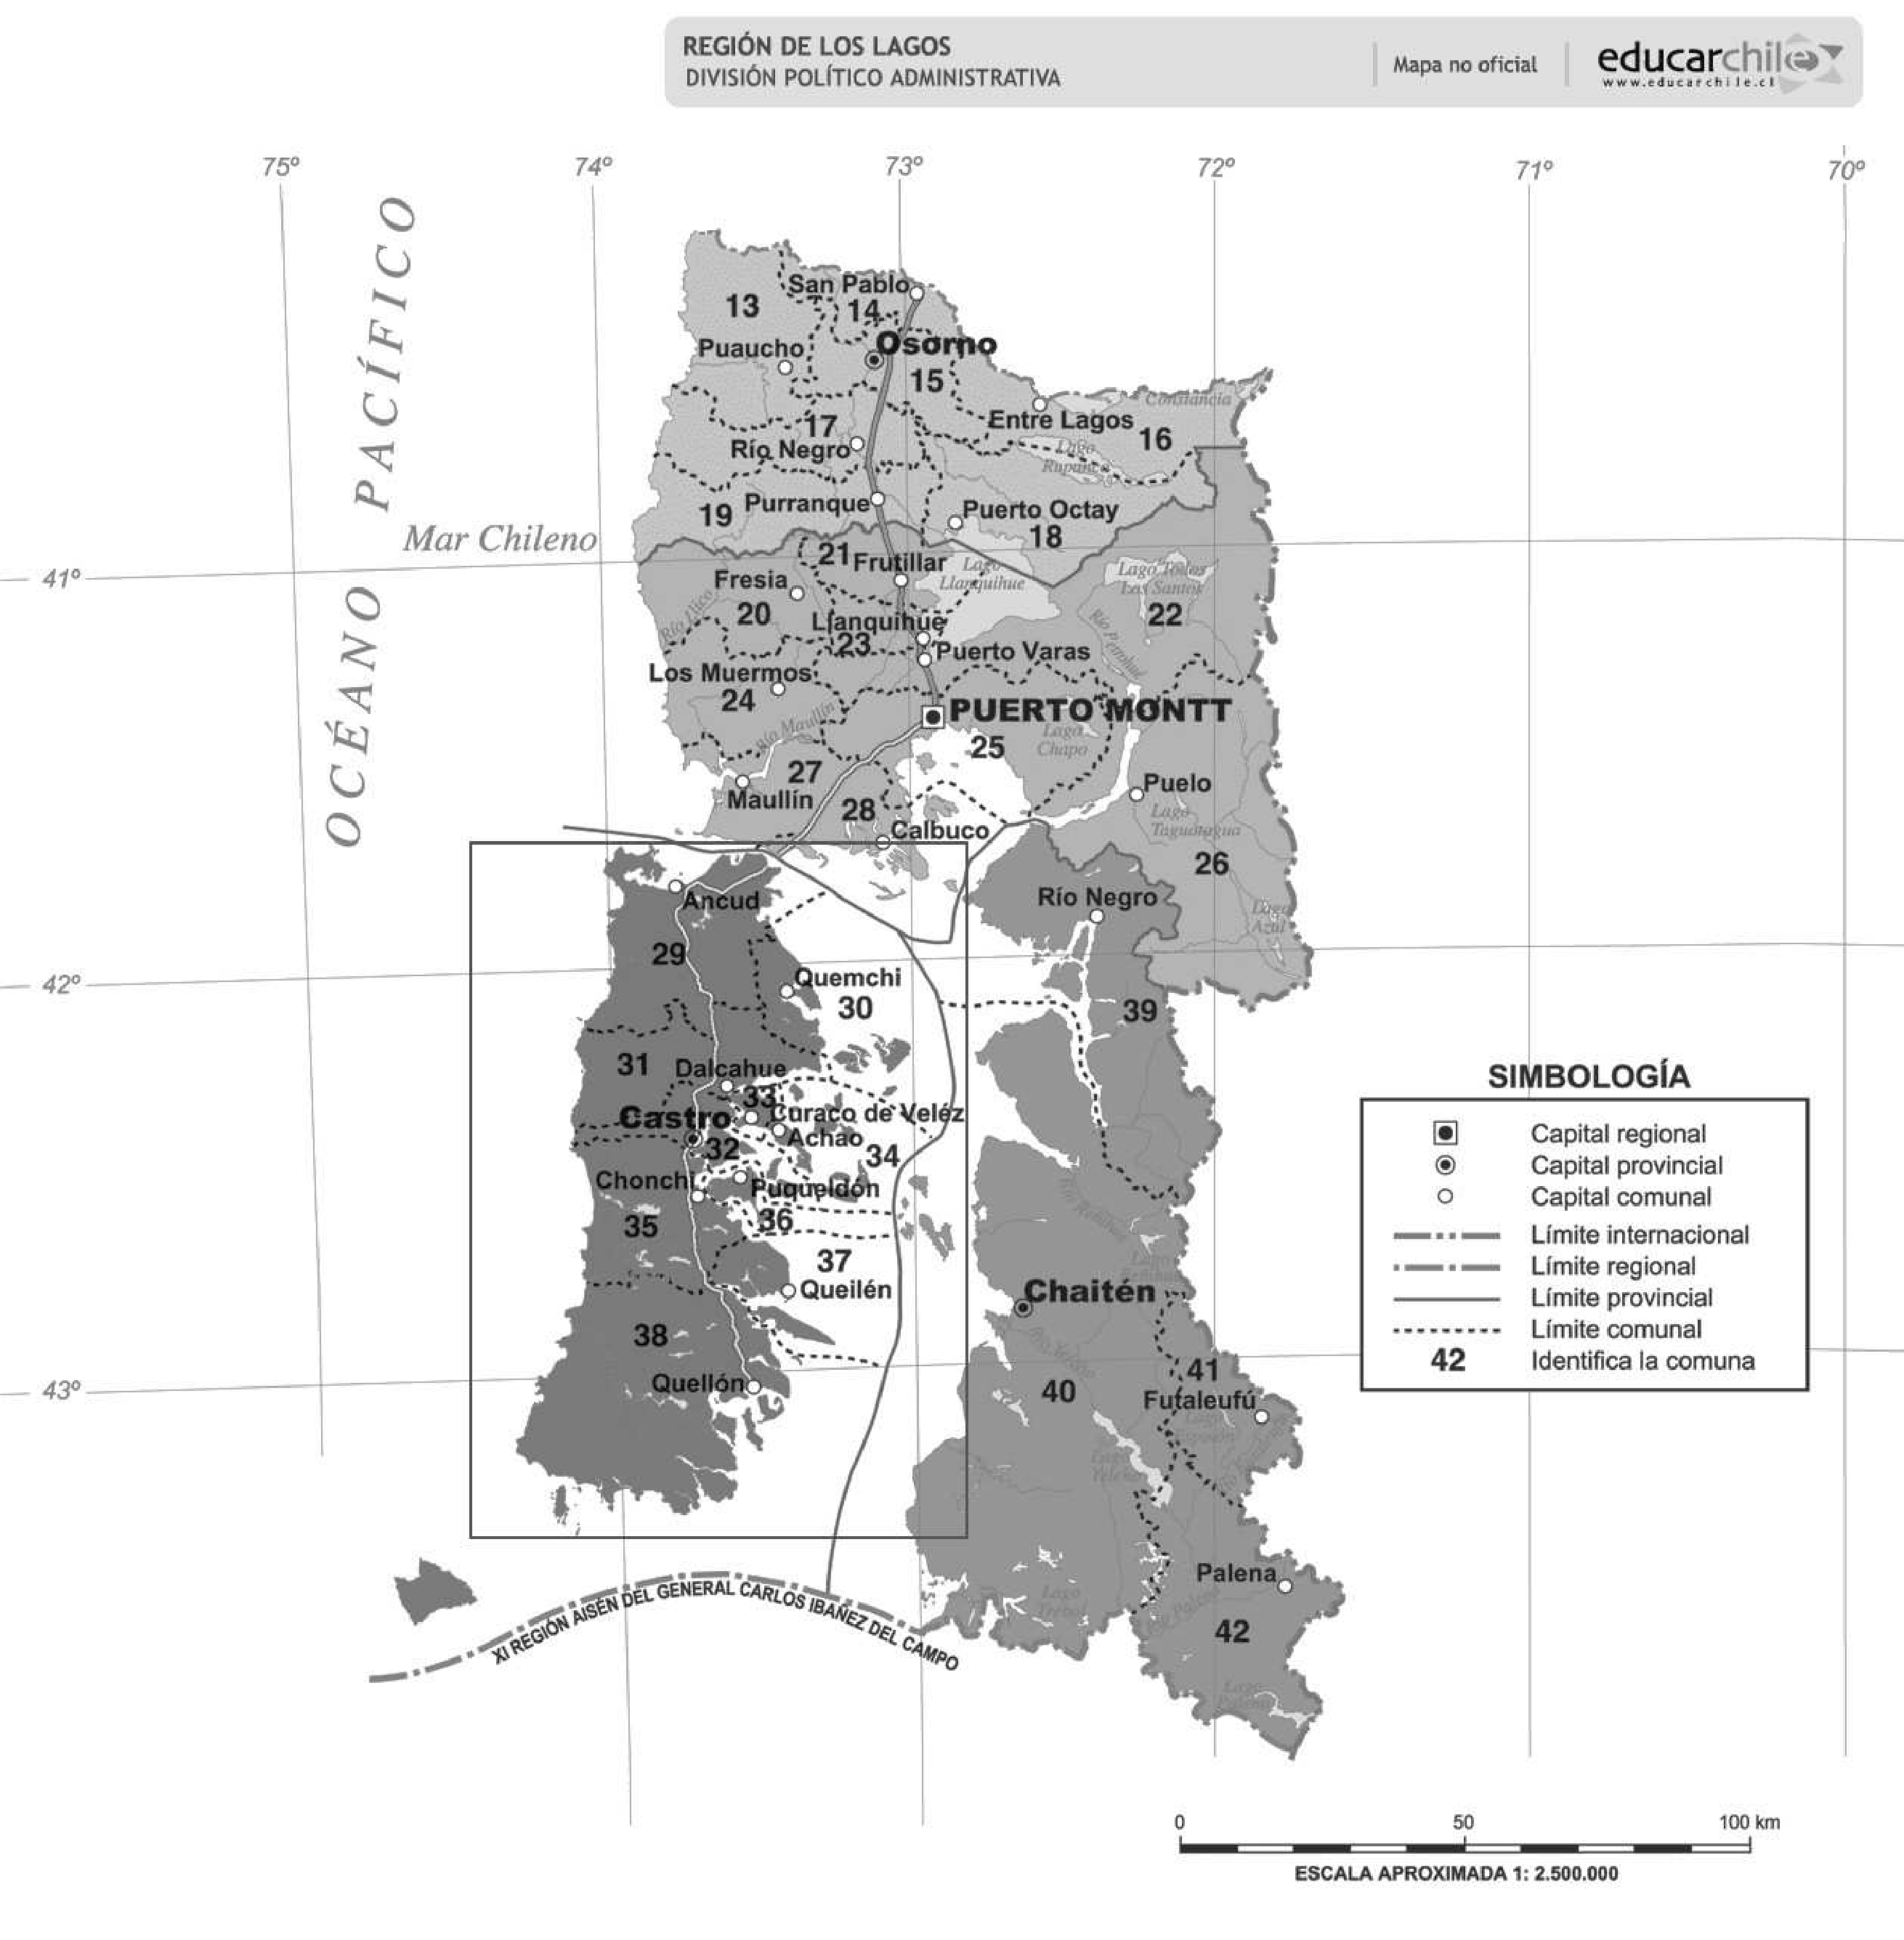
\includegraphics[width=0.5\textwidth]{figure001.pdf}
 \caption{Zona afectada y ubicación geográfica de la Isla de Chiloé.}
 \label{fig01}
 \source{Instituto Geográfico Militar de Chile.}
\end{figure}

La controversia asociada a los hechos giró en torno a la identificación de las
fuentes y responsables de la catástrofe. Los sectores movilizados sostuvieron que estos
correspondieron a salmoneras y organismos gubernamentales, en cuanto al laissez faire
industrial y contaminante en la isla \cite{agenciaefe}. Por el contrario, estos últimos
atribuyeron los hechos al cambio climático, la corriente de El Niño, y la contaminación
costera provocada por la población isleña \cite{infante2016,salmonexpert}. La
movilización fue finalmente contenida mediante el pago de un bono estatal de US\$1.100,
cuyo beneficiario fue la vanguardia del alzamiento, compuesta por sectores de la pesca
artesanal \cite{24horasb}.

La orientación del presente estudio es fundamentalmente empírica. Su objetivo
específico es examinar el rol que asumieron los medios periodísticos durante la crisis
\cite{Mascareo2018b}. Es de interés caracterizar los posicionamientos normativos
subyacentes a la representación con que la televisión abierta chilena cubrió los
acontecimientos. Según la literatura, esta última es objeto de una serie de
cuestionamientos respecto al control que ejerce el gran empresariado local sobre sus
líneas editoriales \cite{cardenas2019,sapiezynska2013}. Al
respecto, ciertos estudios constatan la pérdida de confianza ciudadana sobre la televisión,
principal medio de información en Chile \cite{newman2019}. A ello se suman
protestas de rechazo ciudadano contra su cobertura mediática durante procesos de
conflicto social --concretamente el ‘estallido social’ ocurrido en tal país durante el año
2019 \cite{almeida}.

La axiomatización de la crisis propiciada por los medios de comunicación en Chile,
suele entenderse como expresión de la concomitancia del poder político, económico, y
cultural del gran empresariado \cite[p. 371--395]{palet}. El resultado es un
posicionamiento asimétrico, en los medios abiertos, de las lecturas e interpretaciones
sobre la coyuntura nacional, beneficiando al empresariado sobre el resto de los actores
sociales. Se trata, en resumidas cuentas, de una ‘punta de iceberg’ de la crisis de
legitimidad del neoliberalismo chileno \cite{solimano}. Esta última se evidenció
rotundamente en octubre del año 2019, aunque fue episódicamente evidenciada durante
conflictos menores como el aquí examinado. Los resultados son discutidos desde algunos
elementos fundamentales de las teorías marxistas y luhmannianas \cite{Luhmann1984,marx2003,marx2010,Mascareo2018,wallerstein}.
Por su
flexibilidad, se emplea el análisis del contenido \cite{strauss2002} sobre las
piezas televisivas seleccionadas \cite{eiroa2017,MartnezSalgado2012}. 
A continuación se exponen los aspectos centrales del marco teórico y
esquema de análisis (2), decisiones metodológicas (3), desarrollo (4), y conclusiones (5).


\section{La comunicación de la crisis socioecológica en Marx y Luhmann}\label{sec-lacom}

\subsection{Entendiendo la crisis}\label{sec-crisis}
Para Marx, la crisis en cuanto tal, constituía un momento propio de los ciclos
económicos \cite[p. 11--12]{marx2010}. La era industrial, conformada como resultado de la
emergencia y consolidación del modo de producción capitalista, es portadora de una
multiplicidad de contradicciones. Algunas de ellas son herederas de los modos de
producción anacrónicos —como el esclavismo y feudalismo—, mientras que otras son
originadas en su seno. Por ejemplo aquellas relacionadas a los antagonismos de clase
que la modernidad engendra, descritos como expresión de la contradicción entre el capital
y el trabajo \cite{wallerstein}. También se encuentran elementos
externos y subyacentes, como la incompatibilidad entre la explotación industrial de la
naturaleza y los procesos regenerativos de esta última \cite{Foster2016}. La crisis, por
ende, debe ser examinada en cuanto a las fuentes que la propagan, a modo de diseñar
estrategias orientadas a su intervención o superación. No obstante, es la cuestión del
poder, respecto a la conducción de dicho proceso, el que expresa la centralidad de la
conflictividad entre las clases o grupos sociales en la modernidad democrático-burguesa
\cite{lenin1997}.

Siguiendo sus observaciones e investigaciones desarrolladas en vida, Marx
distinguió que la era industrial modificó sustantivamente la composición de las clases
dominantes en las nuevas formaciones capitalistas. Sustituyendo las clases ociosas --
aristocracia y clero-- por diferentes capas de una clase productiva --burguesías
industriales, comerciales y financieras \cite{marx2003}--, estas fueron capaces de
hegemonizar la conducción de las modernas relaciones de producción. En dicho proceso
los viejos consejeros religiosos de las monarquías fueron prontamente reemplazados por
especialistas técnicos. Haciendo gala de sofisticados métodos científicos, desde entonces
han contribuido a la gobernabilidad y reestabilización del régimen ante períodos de
anarquía \cite{Gunderson2019}. Dichos momentos, exteriorizando la
dualidad entre orden e inestabilidad, flujo y paralización, crecimiento y estancamiento,
desafían las optimistas presunciones burguesas respecto de su modo de producción. La
clase dominante se ve allí empujada a reconocer la imperfección de su sistema, y a
ejecutar acciones rápidas y decididas para conservar sus privilegios \cite{lenin1997}.

Por su aparente reduccionismo, la perspectiva marxista ha sido objeto de múltiples
cuestionamientos provenientes desde el paradigma luhmanniano. Pese a no entregar una
lectura propia y metódica de la crisis \cite{Mascareo2018}, el legado de Luhmann sí
permite comprender sus manifestaciones coyunturales. Para él, la crisis no tendrá una
comprensión unívoca. Aunque sí puede resumirse como un recurso auto-descriptivo,
tendiente a reducir la complejidad propia de los episodios de incertidumbre \cite{Luhmann1984}.
Ejemplos pueden encontrarse en Estados de excepción, revueltas, y/o catástrofes
naturales. Tales coyunturas propicias son para el estudio de la normalidad una vez rota.
Es decir, la crisis remite a lo no-normal, lo no-estable, lo no-certero. Las tareas de re-
equilibrio son encargadas a mecanismos diferenciados funcionalmente. En caso de no
existir, estos deben ser generados oportunamente \cite{Luhmann1991}. Para ello es vital
que la apertura cognitiva logre imponerse sobre la tendencia a la clausura operativa.
Sobre todo en momentos críticos.

La crisis, en dicho esquema, representa también una instancia oportuna para
estabilizar elementos residuales, o desequilibrados, por deficiencias sistémicas anteriores.
Por ejemplo, proliferando, sustituyendo, o perfeccionando acoplamientos estructurales
que permanecen inadecuados \cite{teubner2012}. Tal tarea para Luhmann no reside en
una ‘clase dominante’ o ‘revolucionaria’, sino en los propios sistemas, quienes deben
resolver autopoieticamente sus imperfecciones operativas. Cualquier intromisión exterior
amenaza la integridad de su propia diferenciación funcional \cite{Tkke2010}.
El aprendizaje operativo constituye un mecanismo de evolución sistémica sine qua non.
Sin embargo, en la medida que aumenta la complejidad de los entramados sistémicos, el
desafío es establecer formas de coordinación más simples y complejas. Simples, en
cuanto los sistemas mantengan su autonomía referencial y apertura cognitiva. Y
complejas, en la medida que esto les permita fundar enlaces operativos con formaciones
sistémicas más densas. En resumidas cuentas, la crisis figura como una situación ante la
cual el sistema debe adaptarse evolutiva, flexible, y dinámicamente \cite{Folke2016}.



\subsection{Concebir la comunicación}\label{sec-concebir}
Aunque dedicó años a la labor periodística, \textcite{marx2013} no problematizó
sistemáticamente su carácter en la nueva sociedad capitalista. Han sido sus intérpretes y
lectores quienes han vinculado su legado teórico al análisis contemporáneo de la cultura y
comunicación de masas \cite{mosco2016}. Múltiples trabajos han problematizado
las relaciones entre la producción periodística, y sus contradicciones, con las dinámicas
de la acumulación de valor \cite{Santander2014}. Por ejemplo, respecto a la medida en
que la ideología del capital subsume los contenidos mediáticos del régimen
\cite{sapiezynska2013}. También el modo en que a estas se
contraponen ideológicamente las fuerzas obreras y populares a través de sus propios
medios de prensa. El cine, la televisión, los periódicos y/o radioemisoras serán
concebidas, de tal modo, como arenas de combate ideológico entre las clases. El carácter
de los valores de uso originados por la industria capitalista contemporánea, queda
tensionado por tal disputa. Por ejemplo, si están sujetos operativamente a roles de
reproductores ideológicos, o si bien contribuyen a las modernas dinámicas de consenso
democrático liberal \cite{Habermas2006}.

Lo anterior se encuentra sujeto a cuestionamientos a ser resueltos
situacionalmente, por sobre el principismo que la teoría por momentos puede propiciar. Tal
orientación es correctamente asumida por \textcite{Luhmann1991}, para quien la comunicación
constituye la función operativa central de los sistemas funcionales. Es mediante ella que
estos se revierten de su entorno, bajo un mecanismo de autoreproducción denominado
diferenciación funcional \cite{Tkke2010}. Su despliegue, cognitivamente
abierto y operativamente clausurado, origina infinitos sistemas \cite{billi2017}. 
Cada cual es portador de una codificación específica, articulando un escenario
altamente complejo y contingente. Allí, la coordinación figura como improbable. De ahí la
relevancia de los acoplamientos estructurales, los que posibilitan la armonización de las
expectativas cognitivo-normativas de los sistemas \cite{Luhmann2007}. La función de los
medios de masas es precisamente contribuir a la estabilización de dichos consensos
\cite{becerra2013}.

En cualquier caso, las formaciones sistémicas funcionales coexisten con modos de
diferenciación anteriores, sujeto a lógicas estamentales, o de distinto tipo, herederas del
feudalismo o colonialismo \cite{Mascareo2018}. Estos elementos subsisten en las
confluencias de dominio político y económico, que configuran las élites globales de la era
actual, y constituyen un obstáculo a la distribución democrática del poder. Mediáticamente
esto se observa en la hegemonía ejercida por grandes conglomerados \cite{mosco2016}. 
Ello ha sido denunciado como restricción para el ejercicio de valores democráticos
como derechos a la comunicación y libre expresión \cite{Santander2014,sapiezynska2013}.
Corresponde, desde tal punto de vista, a fuentes de desajuste
entre las expectativas de inclusión que genera la diferenciación funcional, y la exclusión
propiciada por sus propios mecanismos de coordinación. Lo que para el marxismo figura
como una contradicción, para la teoría de sistemas corresponde a una fragilidad de los
sistemas institucionales modernos. Para resolverla no sería necesario superar la sociedad
de clases \cite{lenin1997}, sino la actualización de la configuración general de la formación
sistémica, afín a sus lineamientos funcionales \cite{Luhmann2007,Tkke2010}.



\subsection{Caracterizar lo socioecológico}\label{sec-caracterizar}

La concepción de (la explotación de) la naturaleza ha suscitado múltiples debates
al interior de las corrientes marxistas \cite{arboleda}. Este no se trata de un
problema central en la obra de Marx, lo cual permite entender porqué su abordaje no es
es unívoco ni lineal. También ha sido fuente de polémica la publicación de textos como
‘Dialéctica de la naturaleza’, de Engels, quien parecía prestarle más atención al asunto.
Perspectivas como el ecosocialismo y ecologismo radical han polemizado con las lecturas
que reducen la naturaleza a un mero medio de producción \cite{Foster2016}. Si bien
dichas críticas no son uniformes, su orientación es situar la cuestión ecológica al centro
de la comprensión de la reproducción ampliada del capital. Hablar de ‘antropoceno’ al
interior del marxismo, remite al efecto temporal agregado de la degradación ecológica
impuesta por el capital. A tal elemento remite la categoría de brecha metabólica, ante el
cual las entidades conductoras de la capitalización del plusvalor han tomado un camino
de inacción \cite{Gunderson2019}.

Diferentes son los llamados a la innovación técnica ‘eco-sustentable’ \cite{roman2016}. 
Desde una mirada luhmanniana, la interpelación proveniente de movimientos
sociales, es codificada como búsqueda de soliciones co-evolutivas entre sistemas
humanos y sistema tierra \cite{Folke2016,Luhmann2012}. La intervención
para Luhmann debe pasar por una mediación de discusiones, cuyo resultado será
inevitablemente político. La función de la prensa, así como de los partidos, es la de
contribuir al contraste (democrático) de la colisión (y armonización) de expectativas
\cite{Habermas2006,Luhmann2007}. Pero cada solución a la vez que incluye debe
excluir, por lo que la dificultad de complacer a todas las partes, o de absoluto consenso,
requiere ser abandonada. Lo ecológico no corresponde a una cuestión moral, sino de
supervivencia sistémica. Es posible establecer que las coordinaciones en la materia lleven
adosadas un código que no será el de mejor/peor, o adecuado/inadecuado, sino el de
vital/mortífero.

Esto orienta la particular comprensión de resiliencia entre procesos sociales y
biosféricos para la perspectiva sistémico-luhmanniana. El problema de intervenir se
asume entonces desde la complejización de las relaciones entre ambos \cite{billi2017}.
Allí, la imprevisibilidad de los efectos emanados de la acción humana
figuran como un peligro latente. Por ejemplo, en la implementación de nuevas técnicas o
insumos para los procesos industriales. Al respecto, la evidencia científica suele ser objeto
de polémicas o controversias que objetan la efectividad de ciertas iniciativas. Estas
obstaculizan la adopción de innovaciones, como de ‘energías limpias’. Pero la reiterada
sucesión de episodios de desajuste entre industria y ecosistema sugiere la toma de
acciones oportunas y decididas \cite{Mascareo2018}. Esta es la relevancia de examinar
el contenido y representaciones de las colisiones en contextos de crisis socioecológica
\cite{ValdebenitoAllendes2018}.



\subsection{Esquema de análisis}\label{sec-esquemas}

El marxismo y la teoría luhmanniana de sistemas sociales poseen hoy correlato
decisional en diferentes ámbitos organizacionales. Por ejemplo, sindicatos y movimientos
sociales, así como gobiernos, corporaciones, y agentes técnicos. Considerar el rol de los
medios de comunicación en la irrupción de un conflicto socioecológico, permite examinar
el modo en que los actores comunican sus intereses en la representación de una
coyuntura \cite{Gunderson2019,Habermas2006}. En dicho
proceso, es posible distinguir el modo en que estos diferencian los aspectos materiales a
la base de la crisis. En el caso del ‘mayo chilote’, esto se aprecia entre quienes aludieron
que este se debió a un problema ecológico o social. Vale decir, si la marea roja que
envenenó los mares se propagó por causas humanas o naturales. Tal diferencia cognitiva
deriva en posicionamientos normativos, específicamente sobre el ‘cómo resolver’. Por
ende, analíticamente la crisis puede examinarse desde su comunicación a partir de una
tríada de elementos materiales, cognitivos, y normativos.

A su vez, los procesos de comunicación en las sociedades modernas \cite{Tkke2010},
o de clase \cite{lenin1997,marx2003}, se encuentran atravesados por
asimetrías y relaciones de fuerza de distinto tipo. Esto es reconocido por todas las teorías
sociales \cite{Habermas2006,Luhmann2007,teubner2012}, donde el marxismo y
la teoría de sistemas poseen amplios rendimientos operativos. Ambas teorías conciben la
crisis como un momento de interrupción al curso normal de las relaciones sociales de
producción y comunicación \cite{Luhmann1984,marx2010}. Aquí se ha decidido adoptar
un esquema trifásico para el análisis de la crisis y su comunicación, cuyas partes
integrantes son i) incubación; ii) propagación, y iii) reestructuración \cite{Mascareo2018b}. 
El primer momento remite al período en que germinan y maduran las condiciones
previas al estallido o irrupción de la crisis. Esta situación marca el tránsito de i) a ii). El
período iii) se encuentra dado la aplicación de intervenciones o medidas tendientes a
contener o resolver la propagación de la crisis.

Dado el tiempo transcurrido entre los acontecimientos y la ejecución del estudio, se
ha añadido una fase artificial de iv) ‘pos-reestructuración’. Esta comprende las
comunicaciones de evaluación sobre los hechos de la crisis. Su inclusión en el estudio
responde a una cuestión meramente instrumental. Esto equivale a un intento de trazar el
período de reestructuración como el intervalo dado inmediatamente posterior a la
propagación. Pos-reestructuración se refiere al intervalo comprendido entre los años 2017
y 2020. Allí, se reflexionará a la luz de los acontecimientos, sobre las potencias y límites
de las intervenciones aplicadas para contener la crisis de Chiloé del año 2016. Y especial
atención se dará al impacto operativo real de las propuestas de intervención fundadas en
determinadas corrientes de opinión, fundamentalmente aquellas radicales o ‘hebertistas’.
A continuación se especifican detalles técnicos sobre el diseño metodológico del estudio.



\section{Diseño metodológico}\label{sec-deseno}
El objetivo general del presente estudio es examinar el rol relativo que asumieron
los medios de comunicación de masas durante la crisis del ‘mayo chilote’ del año 2016.
Específicamente, el estudio intenta caracterizar los aspectos normativos subyacentes a la
representación televisiva de los hechos. Según los antecedentes, los episodios de la crisis
fueron abordados por la prensa desde la visibilización, énfasis, y ocultamiento de sus
detalles \cite{cabello2018,ValdebenitoAllendes2018}. Esto por el cruce
de intereses entre ‘información y desinformación’ \cite{cardenas2019,Santander2014,sapiezynska2013}, 
una vez que la prensa es objetada por
la aparente subsunción de sus operaciones a intereses externos. Particularmente,
aquellos promovidos por grupos de influencia política o económica \cite{Habermas2006,Luhmann2007}. 
El examen sigue el esquema analítico descrito en la \Cref{sec-esquemas}.

Como unidad de observación se delimita a comunicaciones publicadas por cadenas
de televisión abierta chilenas, centradas en el conflicto. Estas pueden corresponder a
cápsulas noticiosas, reportajes, entrevistas, despachos en vivo, entre otras. Esta decisión
se fundamenta sobre el reconocimiento de diversos estudios que señalan a la televisión
como el principal medio de información en Chile \cite{newman2019}. Ello no excluye
atender otras fuentes. Siguiendo criterios de complementariedad \cite{strauss2002}, 
se han considerado otros medios periodísticos --como periódicos digitales y notas
en sitios de radioemisoras--, además de informes gubernamentales, reportes científicos,
y artículos académicos sobre el caso de estudio.

El diseño muestral sigue criterios de intención y relevancia, por sobre exhaustividad
\cite{MartnezSalgado2012}. La inclusión y exclusión de unidades muestrales se
orienta por la pertinencia y saturación del material. Esto acorde a medio de comunicación,
y fase de la crisis. De tal articulación se originan casilleros tipológicos, expuestos en la
\Cref{tab01}. Cada casillero busca ser representativo de la articulación de los criterios que lo
originan. En total se hallaron 124 piezas provenientes de cadenas chilenas de televisión
abierta, y 208 de otros medios periodísticos. El método de búsqueda y selección
empleado fue el de bola de nieve. Este arrancó desde los informes gubernamentales,
reportes científicos, y publicaciones académicas. Luego se buscó en plataformas digitales,
como Google y Youtube. La muestra finalmente delimitó a 14 piezas televisivas, y 16
provenientes de otros medios.


\setlength\LTleft{-3cm}
\setlength\LTright{-3cm}
\begin{table}[htpb]
\caption{Diseño muestral.}
\label{tab01}\small
\resizebox{\textwidth}{!}{%
\begin{tabular}{>{\raggedright\arraybackslash}p{0.2\textwidth}llllllll}
\toprule
\multirow{4}{*}{Posiciones en tensión} & \multicolumn{8}{c}{Fase de desarrollo de la crisis} \\
\midrule
 & \multicolumn{2}{>{\raggedright\arraybackslash}p{0.2\textwidth}}{Fase de incubación} & \multicolumn{2}{>{\raggedright\arraybackslash}p{0.2\textwidth}}{Fase de propagación} & \multicolumn{2}{>{\raggedright\arraybackslash}p{0.2\textwidth}}{Fase de} & \multicolumn{2}{>{\raggedright\arraybackslash}p{0.2\textwidth}}{Pos-reestructuración} \\
 & \multicolumn{2}{>{\raggedright\arraybackslash}p{0.2\textwidth}}{Composición muestral} & \multicolumn{2}{>{\raggedright\arraybackslash}p{0.2\textwidth}}{Composición muestral} & \multicolumn{2}{>{\raggedright\arraybackslash}p{0.2\textwidth}}{Composición muestral} & \multicolumn{2}{>{\raggedright\arraybackslash}p{0.2\textwidth}}{Composición muestral}  \\
 & Tv chilena & Otros medios & Tv chilena & Otros medios & Tv chilena & Otros medios & Tv chilena & Otros medios \\
\midrule
Posición causas naturales & 1 & 1 & 2 & 2 & 1 & 2 & 1 & 1 \\
Posición causas industruales & 1 & 1 & 2 & 2 & 1 & 2 & 1 & 1 \\
Debate entre posturas & 1 & 1 & 1 & 1 & 1 & 1 & 1 & 1 \\
\multicolumn{7}{l}{Total:} & \multicolumn{2}{c}{30} \\
\bottomrule
\end{tabular}
}
\source{Elaboración propia.}
\end{table}


Como técnica se empleó al análisis de contenido \cite{eiroa2017},
lo cual involucró descartar análisis semióticos, del discurso, o estadísticos de cualquier
tipo \cite{strauss2002}. No obstante, se sugiere en futuros estudios profundizar
en la comparación de las coberturas mediáticas, empleando estas u otras técnicas. Por
ejemplo, a partir del contraste entre cadenas televisivas y otros medios de prensa, locales
e internacionales. Por el momento, se ha trazado la tarea de generar un insumo de
interpretación flexible y preliminar, desde insumos categoriales fundamentales
provenientes del marxismo y la teoría de sistemas luhmanniana \cite{Luhmann1984,Luhmann1991,marx2003,marx2010,Mascareo2018,wallerstein}.
Específicamente, sobre la sucesión de episodios de crisis, y su respectiva cobertura
mediática \cite{becerra2013,mosco2016,Luhmann2007,marx2013,Santander2014,Tkke2010}.

La cuestión ecológica es también abordada desde ambas teorías sociales
\cite{arboleda,billi2017,Folke2016,Foster2016,Gunderson2019,Mascareo2018b}.
El diferencial
respecto a los estudios sociológicos convencionales, es que el modo de análisis
corresponde más bien a una aproximación interdisciplinar \cite{becerra2014,Osborne2015}.
Esto en cuanto recoge elementos propios del periodismo y ciencias de la
comunicación, en una coyuntura de crisis ecológica \cite{Luhmann2012}. La
presentación de resultados se ejecuta mediante una exposición de representaciones
sobre hechos, y no de la sucesión de hechos en sí. Este camino es exploratorio y
experimental, por lo que aquí se evaluarán sus potencias y límites descriptivos, centrados
en los posicionamientos normativos de la prensa. Los resultados se exponen a
continuación.




\section{Desarrollo}\label{sec-desarrollo}

\subsection{Aspectos generales sobre el ‘mayo chilote’}\label{sec-aspec-generales}
De acuerdo a los antecedentes, la coyuntura estuvo marcada por la colisión de dos
posturas \cite{Mascareo2018b}. Esto en torno a la explicación de la crisis, su
descripción, y fórmula adecuada de intervención. En tal controversia se vieron
enfrentados agentes de la industria acuícola --salmoneras y ‘molusqueras’--, sectores de
la pesca artesanal, población civil, y grupos ambientalistas. El primer actor sostuvo que la
crisis se explica fundamentalmente por una combinación de cambio climático, corriente de
El Niño, y contaminación costera. El conjunto restante de actores presentó un diagnóstico
de unidad. En su primer momento, se sostuvo que la marea roja y varazón tienen su
origen en los efectos residuales de la industria extractiva \cite{roman2016}. Allí, las
autoridades gubernamentales fueron indicadas como cómplices de lo sucedido, al desoír
las recomendaciones emanadas de sus propios informes ambientales, protegiendo los
intereses empresariales. Tras el acuerdo se dividen comunidades y ambientalistas, los
primeros al adherir a la indemnización monetaria, sin reivindicar, negociar, o pactar una
reestructuración productiva de fondo. Esto último marcó el quiebre con los sectores
ambientalistas \cite{ciudadano2016}.

El curso episódico previo a tal desenlace fue el siguiente. Primero, el ‘mayo chilote’
arranca con el decreto gubernamental de prohibición para la extracción y comercialización
de productos marinos \cite{burrows2016}. Tal elemento involucra comprender su origen
desde la historia misma del desarrollo económico de la isla \cite{roman2016}. Este ha
seguido un curso diferenciado respecto a las políticas centrales del país. Solo una vez
introducidas las industrias acuícolas en la zona --a inicios de la década de 1980--, se
transita desde formas económicas de subsistencia hacia un escenario de modernización.
Con el aumento consecuente de la complejidad de las relaciones de producción y cambio
en la isla, se incuban nuevas fragilidades (eco)sistémicas \cite{Mascareo2018,solimano}. 
Parte de ello es el inicio de un ciclo de mareas rojas en el archipiélago
de Chiloé, cuyos primeros registros datan a comienzos de la década del 2000. Para
ciertos científicos esto se explica por la proliferación de procesos de eutrofización y
sobrecarga de nutrientes en el mar, inducidos por la nueva industria \cite{Kamjunke2017,desconcierto}.

Sin embargo, la postura de la industria es sostenida por otras corrientes científicas
\cite{buschmann2016}. La controversia técnica adquiere connotaciones políticas
\cite{cnnchile2016a}. La importancia de ello reside en que el dictamen técnico justificará
un camino de reestructuración a la crisis. De ser afectadas, las salmoneras corren el
riesgo de enfrentar millonarias sanciones e indemnizaciones. La composicipon de la
industria acuícola chilota en principalmente transnacional \cite{roman2016}. Y han
sido empresas japonesas y noruegas las que han financiado buena parte de los estudios
de impacto ambiental locales. Los grupos ambientalistas indican que las empresas se
desembarazan de las recomendaciones emanadas de sus propios estudios \cite{ciudadano2016}. 
También aluden a la necesidad de democratizar el conocimiento,
como forma de evitar la generación de intereses creados en sus procesos de producción
\cite{Gunderson2019}. Esto como parte de la sospecha de que
ciertos estudios sean condescendientes con los intereses de quienes subvencionan sus
investigaciones \cite{tercera}.

La crisis se encuentra marcada por la marea roja, y su combinación con una
inusitada masiva varazón de fauna marina en las costas del sureste de Chiloé. Esta
ocurre específicamente en Cucao, a fines del mes de abril del año 2016 \cite{cnnchile2016b}. 
Los hechos manifiestan la contradicción, o desequilibrio sistémico, entre la
intensidad de los procesos industriales con la regeneración ecológica \cite{Folke2016,Foster2016}. 
Esto facilita la suma de adherentes a las corrientes ambientalistas. Las
movilizaciones irrumpen a lo largo de la isla \cite{24horasa}. A su cabeza se ubican
las familias directamente dependientes de la pesca artesanal \cite{cabello2018}. 
A los pocos días se suman diferentes organizaciones ambientalistas
del resto del país. Estas utilizan sus redes para llamar a protestar en ciudades como
Santiago, Valparaíso y Concepción \cite{agenciaefe}. No obstante, las salmoneras
se mantienen inflexibles en su postura \cite{cooperativa2016}. Por el momento los
medios atienden la represión de Carabineros hacia los manifestantes. La exposición de
pancartas permite a las audiencias reconocer el colaboracionismo entre Gobierno y
empresas transnacionales.

En televisión se exponen los contenidos de los informes de Greenpeace \cite{cnnchile2016b}. 
Estos indican que la fiscalización ambiental en el país ha sido
históricamente deficiente. La orientación gubernamental vigente es señalada como
protectora de las inversiones corporativas transnacionales. Allí, las demandas de la pesca
artesanal han sido sistemáticamente desatendidas, además, sus miembros son
severamente sancionados una vez una vez que incurren en faltas. Son los efectos
sistémicos de una diferenciación funcional concéntrica \cite{Mascareo2018}, o de ‘lado
oscuro’ \cite{teubner2012}. O en términos marxistas, ‘lucha de clases’ \cite{marx2003,marx2013} 
en los planos jurídicos, científicos, y mediáticos. Por su parte las autoridades
manifiestan su preocupación en lo socioeconómico, anunciando medidas pro-laborales
\cite{t13a}. Sin garantías, estas no logran descomprimir las expresiones del
descontento de masas \cite{infante2016}.

Los intentos por acelerar una salida pactada toman forma en la oferta de un bono
para los afectados por la paralización de las actividades marinas \cite{24horasb}. El
primer monto es de US\$150 por familia, pero ante la presión de las calles el acuerdo final
queda en US\$1.100. Dieciocho días transcurrieron previo a la implementación de un
paquete de medidas para la reestructuración del equilibrio de las relaciones económicas
en la isla \cite{quense}. Estas marginan la discusión sobre un programa de transición
hacia una ‘industria verde’. Según analistas, las contradicciones no-encaradas auguran
futuros estallidos en la zona \cite{rios2016}. A continuación se especifica en las acciones
televisivas durante el conflicto.



\subsection{La televisión ante la crisis de Chiloé (2016)}\label{sec-latelev}

Las diferencias entre las coberturas periodísticas del ‘mayo chilote’ se encuentran,
en primer lugar, en la identificación de las fuentes materiales de la catástrofe
\cite{Mascareo2018b}. Esto abre controversias sobre sus elementos cognitivos
(vinculados al debate científico), y normativos (asociados a las fórmulas de intervención
en la materia). El análisis del contenido de las notas, reportajes, despachos en terreno,
entrevistas, y debates televisivos, indica que los hechos son expuestos desde las
posiciones de los actores que los representan \cite{cabello2018}.
La objetividad, como resultado de la aproximación imparcial a un suceso, no es en la
práctica más que una entelequia. Los medios prestan diferenciada atención a la
exposición argumental de las partes \cite{ValdebenitoAllendes2018}.

En televisión, pese a su orientación ‘centrista’, son las lecturas pro-industriales las
que gozan de primacía. Se trata de un elemento transversal entre sus cadenas,
evidenciando para el/la observador/a sólo diferencias de estilo. Pero en lo normativo
operan con homogeneidad, o muy leve heterogeneidad. La oposición es únicamente
movilizada en televisión desde agentes como Greenpeace, cuya estrategias mediáticas
no coinciden con las de aquellos sectores más ‘radicales’ \cite{ciudadano2016}. Tal
exclusión, junto con marcar descontentos y crisis de legitimidad de la televisión en ciertos
sectores, testimonia intencionadas cegueras hacia grupos convencionalmente tildados de
‘extra-parlamentarios’. Al parecer, se les considera demasiado hebertistas, o radicales.
Este maniobrar se corresponde a una toma de partido, en lugar de representar los
acontecimientos desde la multiplicidad de miradas.

La perspectiva pluralista y democrática con que los medios de masas debieran
comportarse en sociedades modernas \cite{Habermas2006}, se pone en práctica como
‘propaganda noticiosa’. Su objeto, en este caso, son los sectores de protesta, tildados
como vandálicos y violentos. Tal elemento es percibido como expresión de la
concomitancia entre poder político y económico de los grupos propietarios de las
comunicaciones en Chile \cite{Santander2014,solimano}. La disputa
comunicacional se da desde la prensa ‘independiente’ \cite{desconcierto}.
Aquellos elementos que los medios convencionales ignoran, son allí puestos en el centro.
Sea por diferenciación funcional \cite{Luhmann2007}, o lucha de clases \cite{marx2013}, se
pone de manifiesto el rol con que los medios de prensa (in)visibilizan la amplitud y
profundidad de los conflictos sociales en Chile.

Lo anterior puede ser entendido a su vez como parte de una línea de fuga ante los
efectos de la concentración del poder mediático de parte de una élite económica
\cite{sapiezynska2013}. Y pese a que ciertas lecturas indican que,
con todo, los medios de masas logran testimoniar las fisuras del régimen \cite{billi2017},
en los hechos el descontento ciudadano hacia ellos no ha
hecho más que incrementar \cite{almeida}. Las distinciones populares sobre
el confinamiento de la apertura cognitiva en los medios de masas \cite{Tkke2010}, 
a manos de las cegueras normativas impuestas por el capital \cite{mosco2016}, 
ha contribuído a la crisis actual de los medios en Chile. Sobre ella urge su
democratización \cite{cardenas2019}, lineamiento que queda aquí esbozado como
sugerencia para futuras aproximaciones. A continuación se detalla el análisis fásico de
estos elementos.



\subsection{La fase de incubación}\label{sec-fase-incu}

Del análisis del material empírico se entiende que la exposición de los hechos que
marcan la crisis varía según su fase de desarrollo. Durante la incubación, que va desde
inicios de marzo hasta fines de abril, la cobertura se limita a cápsulas noticiosas
\cite{burrows2016}. Allí, se exhiben declaraciones de científicos, autoridades
gubernamentales, dirigentes sindicales, pescadores artesanales, y comerciantes del
sector. Cada actor expone sus posturas e intereses, sobre los acontecimientos que para
algunos auguran la sucesión de una catástrofe ecológica. Si bien en general las
declaraciones televisadas se entrelazan desde la perspectiva de la naturalidad de los
ciclos de marea roja \cite{cabello2018}, en otros medios se
proyectan balances más alarmistas \cite{desconcierto}. Estos últimos
problematizan la desregulación sobre la industria, y la adulteración que esta induce a los
procesos de regeneración ecosistémica.

Por el momento tales antecedentes no figuran en medios televisivos, siendo
atendidos someramente sólo por ciertos periódicos convencionales \cite{tercera}.
Por el contrario, en televisión las comunicaciones se limitan a señalar que prima un clima
de colaboración entre agentes gubernamentales, empresariales, comunitarios, y
sindicales, para enfrentar colectivamente los efectos de la crisis \cite{burrows2016}.
Transversal es la preocupación sobre los efectos socioeconómicos generados por la
paralización de los procesos de reproducción ampliada del capital en la zona. Se teme
que estos sean descargados sobre la clase trabajadora, confirmando la contradicción
entre el carácter social de la producción y la apropiación privada de sus beneficios
\cite{wallerstein}.

La prensa habla de riesgos de aumento en las tasas de desempleo. Más aún, la
crisis ocurre en medio del período de mayor auge comercial en la zona. Este corresponde
a la víspera de ‘Semana Santa’, donde los pescados y mariscos chilotes son exportados
hacia el resto del país. También señalan que autoridades y científicos temen la
proliferación de un foco infeccioso en la isla \cite{nunez}. Las conversaciones que
salen a la luz pública sirven como base para el diseño de un paquete de ayuda. Los
noticieros no profundizan al respecto. Para la teoría luhmanniana, el hecho de comunicar
involucra un paradójico ejercicio de inclusión excluyente. Al momento que se observa
algo, se omite otra cosa \cite{becerra2013,Luhmann2007}. Se trata de una
lectura donde se asume que la comunicación es incapaz de ‘integrarlo todo’.

Al margen de justificaciones, los medios de masas adhirieron durante la primera
fase de la crisis, a la lectura esta se originó por un ciclo natural de marea roja
\cite{Kamjunke2017}. Esto marginó de la pantalla a quienes sostuvieron argumentos
contrarios, que indican que dicho ciclo se origina por la introducción de una actividad
industrial desregulada \cite{ciudadano2016}. En último término, se trata de una
clausura operativa cuyo eje es normativo. Por sobre seguir lineamientos básicos de
pluralismo informativo \cite{Habermas2006}, evidencia signos de instrumentación política
de parte de grupos de influencia económico-política \cite{sapiezynska2013}. En la
práctica, el lado oscuro de la diferenciación funcional logra imponerse \cite{teubner2012}.
Esto en un escenario donde ampliamente estudiado se encuentra la primacía del mundo
económico sobre el resto de los ámbitos sociales \cite{palet,solimano},
fuente de descrédito del modelo chileno y sus medios de comunicación \cite{almeida,cardenas2019}.

Apropiada es en tal contexto la distinción de lucha de clases mediática, posible de
exteriorizar mediante el contraste periodístico \cite{desconcierto,tercera}. 
Para Marx los episodios de crisis permitían evidenciar el movimiento contradictorio
de la sociedad capitalista \cite{marx2010}. El que la prensa abierta tome partido por
determinadas posiciones, que son antagónicas con otras, no debiera extrañar en un clima
de autoritarismo. Por ejemplo, el propiciado por una dictadura. Pero en momentos donde
las libertades democráticas se encuentran resguardadas jurídicamente, dicho
comportamiento es problemático. Así lo han denunciado diferentes estudios
internacionales sobre la situación de la libertad de expresión en el mundo subdesarrollado
\cite{newman2019}.

En este caso, a través la prensa el empresariado parece ensalzarse a sí mismo
como intérprete y gestor de la crisis. En sus (auto)representaciones mediáticas, sus
intereses figuran como apolíticos, objetivos, y científicos \cite{mosco2016},
aludiendo a que ‘la catástrofe no es capitalista, sino ecológica’ \cite{Foster2016,Gunderson2019}. 
Tal elemento será puesto en entredicho por el
conjunto de organizaciones obreras, territoriales, y ambientalistas, enfrentadas a las
fuerzas de un régimen de apariencia corporativista en Chiloé \cite{Mascareo2018b,ValdebenitoAllendes2018}.


\subsection{La propagación de la crisis}\label{sec-prop-crisis}
Esta fase arranca con la masiva varazón de fauna marina en las costas de Cucao
\cite{Mascareo2018b}, seguida de un estallido social en la isla \cite{cabello2018,ValdebenitoAllendes2018}.
Este involucra cortes de ruta,
barricadas, y enfrentamientos entre manifestantes y fuerzas de orden \cite{24horasa,t13a}. 
En dicho momento, la televisión aumenta significativamente la cobertura de
los hechos. Allí, tiende a ponerse en evidencia la posición político-normativa con que
ejecuta su cobertura. Lo que prontamente será nombrado como ‘mayo chilote’, es ahora
objeto de discusión en espacios de debate político, matinales, y ‘talk shows’ \cite{cnnchile2016b}.
Las declaraciones de miembros de la comunidad científica adquieren especial
relevancia. Sólo gozan de tribuna quienes adhieren a la lectura de la ‘naturalidad de la
marea roja’. Los que esgrimen argumentos contrarios a la industria acuícola, son
marginados hacia medios escritos y/o radiales, preferentemente digitales \cite{ciudadano2016}.

Como se ha sostenido, tales marginaciones han servido para inducir la actual crisis
de legitimidad de los medios de masas en Chile \cite{newman2019,solimano}. 
Específicamente, la sistemática exclusión de voces del descontento social. Por
ejemplo, aquellas sobre el modo de gobernar heredero de la dictadura, y perpetuada con
la transición tutelada \cite{palet,Santander2014,sapiezynska2013}.
Así y todo, se constatan ciertas líneas de fuga en la cobertura televisiva
de las protestas en Chiloé \cite{billi2017}. La exhibición de lienzos y
pancartas permite exteriorizar parte del contenido de la disconformidad ciudadana con el
extractivismo \cite{Gunderson2019}. Las declaraciones de los/as
manifestantes en pantalla hablan de una generalizada sospecha de que la catástrofe pudo
ser evitada, de haberse tomado medidas oportunamende \cite{24horasa,decima2016}.

Pero la falta de claridad científica genera un escenario de crisis mimética \cite{girard216}, 
cuyo chivo expiatorio será prontamente identificado con la divulgación de imágenes
de un exuberante vertimiento de salmones muertos al mar \cite{agenciaefe}. Pese a
que ciertos científicos le restan importancia al hecho \cite{buschmann2016}, este
permite argumentar a favor de la tesis ambientalista. Greenpeace adquiere gran atención
televisiva \cite{cnnchile2016b}. Sus portavoces indican que el vertimiento vulnera normas
de derecho ambiental nacional e internacional vigente. También aluden a una
combinación de factores climáticos --calentamiento global, corriente de El Niño-- con
acciones humanas --adulteración ecosistémica a manos de la explotación marina
\cite{Kamjunke2017}. Salmoneras y pescadores artesanales se culpan
recíprocamente. Estos últimos en televisión exclaman “el mar ha muerto”.

Los medios cubren los anuncios gubernamentales de ayuda económica para los
afectados directos de la crisis. Se habla de un bono de US\$150. Pero en las calles las
manifestaciones se intensifican \cite{24horasa,infante2016}. La discusión política
sobre el ‘qué hacer’ copa la cobertura. Los sectores conservadores llaman al orden y
deponer las movilizaciones \cite{agriculturatv}. Su lectura se centra en que estas
profundizan la crisis, cuando se requiere reactivar el ciclo económico de la isla. Políticos
progresistas sostienen que la situación debe ser evaluada. Lo importante, señalan, es
proteger a las familias más vulneradas por la catástrofe \cite{cooperativa2016}. En
paralelo, pescadores y activistas suman adherentes. Se realizan actos de apoyo a la
movilización chilota en otras ciudades del país --como Santiago, Valparaíso y Concepción
\cite{agenciaefe}. La prensa internacional, y ciertos medios locales de ‘prensa
alternativa’, exhiben con mayor atención las posturas contrarias a la industria salmonera
\cite{Mascareo2018b}.

La televisión chilena hegemoniza una condena hacia las protestas, en tanto
expresiones de violencia y vandalismo \cite{cabello2018}. Su
preocupación central es la de erigir la necesidad de disipar dudas científicas sobre la
varazón, y fortalecer el sistema laboral de Chiloé \cite{infante2016}. En los medios
comienza a adquirir notoriedad un proyecto de reconversión para la isla. Este es
promovido por una alianza corporativo-gubernamental. Su énfasis es industrializar los
sectores agrícolas y de servicios. Mientras tanto, el monto ofrecido por el Gobierno para
deponer las movilizaciones aumenta a US\$1.100. Este logra dividir a los sectores
movilizados, entre quienes requieren urgentemente una solución económica, y
aquellos/as que apelan a reformas estructurales \cite{quense}. También figura una
fantasmagórica entrada de sectores reaccionarios. Estos se compondrían por
transportistas, respaldados por población civil afectada por el desabastecimiento, y
uniformados \cite{decima2016,t13a}. El episodio de la lucha ecológica y de
clases se sella, aparentemente, en Chiloé \cite{Foster2016,ValdebenitoAllendes2018}.



\subsection{La reestructuración tras el conflicto}\label{sec-reestr-conflicto}

Finalmente, dieciocho días transcurrieron hasta el triunfo del acuerdo entre
gobierno y sectores movilizados. Dicho hito inicia la fase de reestructuración de la crisis
en Chiloé (2016). Hasta el momento la televisión seguía de cerca el transcurso de las
negociaciones. Sobre las causas de la varazón, se determina que serán órganos expertos
los que entregarán su veredicto \cite{24horasb}. La cobertura televisiva se centra en
los aspectos que condicionan el pago del bono. Por ejemplo, ser trabajador vinculado al
sector pesquero, poseer registro vigente, haber tenido descargas asociadas a los
productos afectados --como machas, cholgas y choritos--, y no contar con otros
ingresos. El beneficio aplica para pescadores, buzos, asistentes, recolectores de orilla (o
algueros), y patrones de embarcación.

La prensa afín a las posiciones empresariales presta atención a las pérdidas
monetarias de la industria a raíz de las movilizaciones \cite{emol,salmonexpert}.
En ‘medios independientes’ dicha señal se codifica como preámbulo de despidos
en la industria, acompañados de automatizaciones, y/o deslocalizaciones productivas. En
sus análisis sobre las transiciones históricas entre los modos de producción, \textcite{marx2010}
constata que durante la era industrial, la economía política se consolida como sostén
ideológico de la clase dominante. Tal disciplina será la fuente de las axiomatizaciones
coyunturales realizadas por la burguesía, desplazando a la religión propia de los tiempos
monárquico-feudales. En el caso del ‘mayo chilote’ la Iglesia católica jugó un rol mediador.
Pero fue la monetización la que finalmente logró imponerse.

Sistémicamente, lo anterior expresa la consolidación del dinero como medio de
comunicación simbólicamente generalizado \cite{becerra2013,Luhmann1991}.
Pero tal lineamiento no está exento de fragilidades \cite{Habermas2006}.
Desembarazarse de las contradicciones principales, a saber, ecológicas y sociales,
sustenta las fuentes para la reiteración de episodios similares o de mayor envergadura en
el futuro \cite{Folke2016,greenpeace}. El debate sobre la incompatibilidad entre
industria y naturaleza es retomado reiteradamente en la era contemporánea \cite{ciudadano2016,Foster2016}.
Y sobretodo a propósito de la irrupción de
acontecimientos que abren la discusión sobre su actualidad. No obstante, pese a que
iniciativas como la agroecología tomen fuerza \cite{arboleda}, en los hechos se ha
consolidado la estrategia de solución gradual y reformista \cite{rios2016}.

El debate científico no corroboró si la catástrofe de Chiloé se debió a causas
industriales \cite{t13b}. Quienes insistieron en que el fenómeno se debió a una marea
roja, recomendaron paralizar las actividades marinas por tres meses. Quienes sostuvieron
que la catástrofe se explica por una sobrecarga bioquímica de los mares, aluden a la
necesidad de implementar un proceso de paralización total. Esto hasta contar con
evidencia que indique el avance de una restauración o regeneración significativa \cite{nanjari}.
No es difícil anticipar que la segunda posición fuera tildada de ‘inviable’ o
‘demasiado radical’ por los órganos de toma de decisiones \cite{Gunderson2019}.
Tal clausura se justifica en proyectos, sin garantías, de implementar
medidas de ‘industria verde’ \cite{Folke2016}.

Una vía con ‘vocación de neutralidad’ hubiera indagado en las responsabilidades
de lo sucedido. Por ejemplo, encargando investigaciones a órganos imparciales --
internacionales probablemente. Pero en lugar de ello se observó una concomitancia entre
capital salmonero y centros de investigación que publicaron conclusiones prácticamente
‘hechas a la medida’ \cite{buschmann2016}. El accionar de los hebertistas ecológicos
tampoco ha conducido a la politización de masas sobre las causas ambientales. Sus
acciones no han ido más allá de lo testimonial, siendo necesaria la inducción de una
reflexión profunda, conducente a la codificación popular de la cuestión ecosistémica. El
camino permanece abierto, así como la lucha por el porvenir ecológico de Chiloé y el
mundo \cite{ValdebenitoAllendes2018}.


\subsection{Pos-reestructuración}\label{sec-pos-reestr}

La implementación de las medidas de contención al conflicto de Chiloé evidenció
sus contradicciones a los pocos meses. Nuevos episodios de marea roja se presenciaron
en la isla \cite{24horasc}. También el seguimiento televisivo de los hechos distó de ser
unívoco. De una parte se destaca que la reestructuración ejecutada por el gobierno fue
insuficiente \cite{t13c}. Las tendencias a la pauperización sobre la vida de la población
se desplegaron al alza. Indicador de ello es la constatación de un aumento de las
ocupaciones irregulares de terrenos, o ‘tomas’. El que la discusión científica sobre la
varazón no entregara un veredicto concluyente, deslegitima su propio accionar,
abriéndose debates sobre el control del conocimiento en Chile. Ciertos espacios
televisivos dan tribuna, en este período, a técnicos ambientalistas. Estos señalan que ante
la catástrofe del 2016 las salmoneras decidieron migrar a otras zonas patagónicas,
eludiendo el costear daños ambientales \cite{gonzalez2017}.

Ante las externalidades negativas para la actividad acuícola en el Golfo de Chiloé,
la prensa afín a la industria había realizado tal anuncio con anterioridad \cite{gonzalez2016,infante2016,salmonexpert}.
Las tesis fundamentales del
extractivismo y del antropoceno tienden a ser corroboradas \cite{Foster2016,Gunderson2019}.
Pero la lectura televisiva enfatiza en los
costos socioeconómicos de la movilización \cite{24horasc}. Esto dado que los índices
de desempleo han aumentado, y que quienes se desempeñaban bajo regímenes de
trabajo diario --como pescadores y recolectores de orilla-- no lograron ser reabsorbidos
por las políticas de ‘reconversión laboral’. Pero la televisión sostiene que la pobreza tiene
su lado amable, facilitando la proliferación de lazos comunitarios y ‘ollas comunes’.
También señalan que tras la catástrofe se generaron mecanismos de anticipación y
contención ante nuevos episodios similares, lo cual contrasta con las nuevas mareas rojas
\cite{galaz2016,Kamjunke2017}.

La publicación de registros audiovisuales realizados por activistas ambientales
entrega nuevos antecedentes sobre la crisis chilota del 2016 \cite{quense}. Estos se
posicionan desde el interior de las manifestaciones, ilustrando la significación de las
luchas ecológicas y de clase en el sur de Chile. Allí, la población figura consciente del
poder de influencia de la industria. Esto sobre la totalidad de los elementos del régimen,
como gobierno y autoridades, medios de comunicación, policía, centros científicos, y
tribunales. Por sobre redistribuir el poder, vía inclusión y/o participación \cite{Folke2016,Mascareo2018b}, 
las comunidades lo reivindican en sí y para sí \cite{marx2003}. Las tesis leninistas \cite{lenin1997}, sobre la toma del poder del Estado, para
reestructurar y/o originar la sociedad nueva, se mantienen históricamente vigentes. Estas
subyacen a las discusiones contemporáneas sobre la conducción de los procesos
transicionales de salida a las múltiples manifestaciones de la crisis del capitalismo
contemporáneo \cite{arboleda}. A la luz de los antecedentes aquí descritos, el
proyecto de la crítica de la economía política \cite{marx2010}, tendiente a la construcción
de la sociedad nueva, se mantiene abierto.



\section{Conclusiones}\label{sec-conclusiones}

El análisis presentado posibilita problematizar el rol que asumen los medios de
comunicación de masas durante el desarrollo de una coyuntura de crisis socioecológica.
Como unidad de observación se ha considerado principalmente la cobertura televisiva
abierta del ‘mayo chilote’ del año 2016. A modo de complementariedad, se ha triangulado
tal fuente de información con coberturas realizadas por otros medios de prensa, artículos
académicos, e informes científico-gubernamentales. La técnica de investigación empleada
complementa elementos del análisis de contenido y coyuntural. La distancia temporal
entre la ocurrencia de los hechos y la ejecución del estudio, permite someter a la prueba
de la verificación histórica la validez de ciertas tesis enunciadas por agentes claves en
conflicto. Esto ha permitido determinar que los enunciados de ‘ambientalistas radicales’
estuvieron en lo cierto en el pronóstico de nuevas mareas rojas si no se intervenía
decididamente en sus fuentes. Sin embargo, su debilidad radica en el fracaso emanado
de sus tácticas políticas, lo cual es necesario de investigar a posterioridad.

El estudio del conflicto en cuanto crisis, se ha desarrollado integrando las teorías
sistémicas --de orientación luhmanniana-- y marxista. Esto ha facultado para reconocer
que a la conducción del proceso de intervención sobre la crisis subyacen conflictos de
poder e influencia entre diferentes agentes. En el caso estudiado, se trata de una alianza
empresarial-gubernamental la que hegemoniza dicho proceso. Esto en detrimento de
otros actores, como comunidades rurales, sindicatos, y organizaciones ambientalistas. Tal
distinción se puede problematizar desde categorías como lucha de clases y diferenciación
funcional concéntrica. La reflexión comparativa sobre las potencias y límites de cada una
se ha desplazado para futuros análisis. Por el momento se ha intentado esbozar la
posibilidad de su integración, o compatibilidad, desde una mirada interdisciplinaria entre
ciencias sociales y de la comunicación. Con todo, desde tal posición se ha destacado que
a la base de la crisis y su intervención se encuentra la cuestión del poder, lo que debiera
ser también objeto central de futuras aproximaciones.

Lo anterior influye decididamente sobre el desarrollo operativo de las funciones
periodísticas en la cobertura de procesos de crisis y/o conflicto social. De acuerdo a las
observaciones, esta queda subsumida por la orientación normativa prevaleciente entre el
o los grupos propietarios de los medios. En el caso de la televisión abierta chilena,
ampliamente estudiadas se encuentran las fragilidades propias de su modelo de
propiedad oligopólico, cuyo autoritarismo y control quedan aquí advertidos. Aún así se
requiere profundizar sobre los matices con que las cadenas de televisión atienden los
conflictos sociales en Chile. Aquí se ha sostenido que estos tienen que ver con cuestiones
de estilo por sobre contenido. Es necesario aplicar otras técnicas de análisis que permitan
lograr distinciones más profundas en la materia. Por ejemplo, contrastes estadísticos de
contenidos entre diferentes medios, semióticos de la imagen, entre otros.

El esquema de análisis de los procesos de crisis y su comunicación, basado en la
diferenciación de sus fases --incubación, propagación, y reestructuración-- y elementos
--materiales, cognitivos, y normativos--, ha resultado pertinente. Se destacan
principalmente sus potencias en cuanto a la flexibilidad, apertura, y adaptabilidad para el
examen de diferentes tipos de conflictos o controversias. Dichas características permiten
aplicarlo siguiendo variadas combinaciones analíticas, sean teóricas o metodológicas. En
el presente caso ha mostrado óptima afinidad con el caso de estudio, y perspectivas de
análisis interdisciplinarias, como lo son el marxismo y la teoría de sistemas luhmanniana.
También ha resultado pertinente la distinción dual de ‘énfasis y cegueras’ sobre la
comunicación periodística. Principalmente en cuanto a la determinación de sus
orientaciones normativas. Esto ha quedado en evidencia en el modo de presentación con
que los medios cubren los hechos de un determinado conflicto o controversia. Pero se
requieren futuras observaciones empíricas que contribuyan a corroborar hasta qué punto
estos insumos evidencian potencias y/o fragilidades.




\printbibliography\label{sec-bib}

\end{document}
